% Created 2024-01-10 mié 19:38
% Intended LaTeX compiler: pdflatex
\documentclass[aspectratio=169, usenames,svgnames,dvipsnames]{beamer}
\usepackage[utf8]{inputenc}
\usepackage[T1]{fontenc}
\usepackage{graphicx}
\usepackage{longtable}
\usepackage{wrapfig}
\usepackage{rotating}
\usepackage[normalem]{ulem}
\usepackage{amsmath}
\usepackage{amssymb}
\usepackage{capt-of}
\usepackage{hyperref}
\usepackage{color}
\usepackage{listings}
\usepackage{mathpazo}
\usepackage[spanish]{babel}
\usepackage{gensymb}
\usepackage{amsmath}
\usepackage{diffcoeff}
\usepackage{steinmetz}
\usepackage{mathtools}
\bibliographystyle{plain}
\usepackage{siunitx}
\sisetup{output-decimal-marker={,}}
\DeclareSIUnit{\watthour}{Wh}
\hypersetup{colorlinks=true, linkcolor=Blue, urlcolor=Blue}
\usepackage[symbol, perpage]{footmisc}
\newcommand{\laplace}[1]{\mathbf{#1}(\mathbf{s})}
\newcommand{\slp}{\mathbf{s}}
\newcommand{\fasor}[1]{\mathbf{#1}(\omega)}
\newcommand{\atan}{\mathrm{atan}}
\parskip=5pt
\usetheme{Boadilla}
\usecolortheme{rose}
\usefonttheme{serif}
\author{Oscar Perpiñán Lamigueiro}
\date{}
\title{Fundamentos de Electrotecnia}
\setbeamercolor{alerted text}{fg=blue!50!black} \setbeamerfont{alerted text}{series=\bfseries}
\AtBeginSubsection[]{\begin{frame}[plain]\tableofcontents[currentsubsection,sectionstyle=show/shaded,subsectionstyle=show/shaded/hide]\end{frame}}
\AtBeginSection[]{\begin{frame}[plain]\tableofcontents[currentsection,hideallsubsections]\end{frame}}
\beamertemplatenavigationsymbolsempty
\setbeamertemplate{footline}[frame number]
\setbeamertemplate{itemize items}[triangle]
\setbeamertemplate{enumerate items}[circle]
\setbeamertemplate{section in toc}[circle]
\setbeamertemplate{subsection in toc}[circle]
\hypersetup{
 pdfauthor={Oscar Perpiñán Lamigueiro},
 pdftitle={Fundamentos de Electrotecnia},
 pdfkeywords={},
 pdfsubject={},
 pdfcreator={Emacs 29.1 (Org mode 9.6.11)}, 
 pdflang={Spanish}}
\begin{document}

\maketitle

\section{Conceptos Fundamentales}
\label{sec:org0341f48}
\begin{frame}[label={sec:org6b7937d}]{Tensión Eléctrica}
El \alert{potencial eléctrico en un punto}, \(v(t)\),  es la energía potencial que tiene una carga unitaria en ese punto debida al campo eléctrico. 

\begin{center}
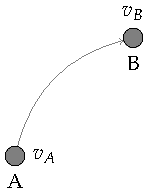
\includegraphics[height=0.3\textheight]{../figs/tension_puntos.pdf}
\end{center}

La \alert{tensión o diferencia de potencial entre dos puntos} A y B, \(u_{AB}(t)\), es el trabajo realizado por el campo eléctrico al desplazar una carga unitaria entre esos puntos. 

\begin{equation*}
  u_{AB}(t) = v_A(t) - v_B(t) = \frac{dW_{e}}{dq}
\end{equation*}

La \alert{unidad} de la tensión eléctrica es el \alert{voltio} (V).
\end{frame}

\begin{frame}[label={sec:orgcb96763}]{La trayectoria no importa}
Dado que el campo eléctrico es \alert{conservativo}, la diferencia de potencial entre A y B \alert{no depende de la trayectoria} seguida para realizar el desplazamiento, sino únicamente del potencial existente en cada uno de los puntos. 

\begin{center}
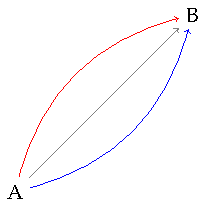
\includegraphics[height=0.6\textheight]{../figs/diagrama_tension.pdf}
\end{center}
\end{frame}

\begin{frame}[label={sec:orge415b95}]{El signo depende del sentido}
Aunque la trayectoria no sea relevante para el cálculo de la tensión, siempre hay que tener en cuenta el \alert{sentido del desplazamiento}. 

\begin{center}
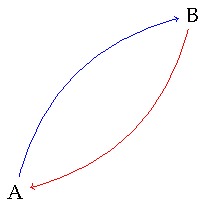
\includegraphics[height=0.4\textheight]{../figs/sentido_tension.pdf}
\end{center}

Así, si el movimiento se produce desde B hasta A obtenemos el signo contrario al anterior resultado:

\begin{equation*}
  u_{BA} = v_B - v_A = - u_{AB} 
\end{equation*}
\end{frame}

\begin{frame}[label={sec:orgddc8056}]{Corriente Eléctrica}
Se define la \alert{intensidad de la corriente eléctrica} como la variación de la carga \(q(t)\) que atraviesa la sección transversal de un conductor por unidad de tiempo:

\begin{equation*}
  i(t)=\frac{dq(t)}{dt}
\end{equation*}

\begin{center}
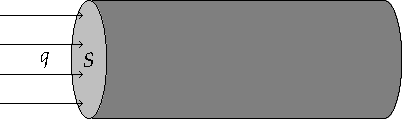
\includegraphics[height=0.2\textheight]{../figs/seccion_conductor.pdf}
\end{center}

La corriente eléctrica se produce por el \alert{movimiento de los electrones libres} que fluyen por el conductor. Sin embargo, por razones históricas, el \alert{convenio} que se se emplea considera como sentido de la corriente el debido al \alert{movimiento de las cargas positivas}.

La \alert{unidad} de la corriente es el \alert{amperio} (A).
\end{frame}

\begin{frame}[label={sec:orgb8f6ca9}]{Potencia Eléctrica}
La \alert{potencia eléctrica} es la variación del trabajo del campo eléctrico por unidad de tiempo:

\begin{equation*}
  p(t)=\frac{dW_{e}}{dt}
\end{equation*}

Esta definición genérica puede relacionarse con las anteriores variables:

\begin{align*}
  p(t) &= \frac{dW_e}{dq} \cdot \frac{dq(t)}{dt}\\
       &= v(t)\cdot i(t)
\end{align*}

La \alert{unidad} de la potencia eléctrica es el \alert{vatio} (W).
\end{frame}

\begin{frame}[label={sec:org60d0f09}]{Signo de la potencia eléctrica}
Para determinar el \alert{signo de la potencia eléctrica} hay que tener en consideración los signos de las variables de las que depende, la tensión y la corriente. 
\begin{itemize}
\item Cuando las flechas de ambas variables tienen el \alert{mismo sentido} la potencia eléctrica es \alert{positiva}
\item Cuando las flechas tienen \alert{sentidos opuestos} la potencia eléctrica es \alert{negativa}.
\end{itemize}

\begin{center}
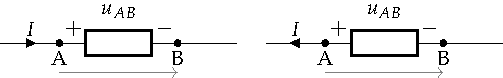
\includegraphics[height=0.2\textheight]{../figs/signo_potencia.pdf}
\end{center}
\end{frame}

\begin{frame}[label={sec:orgb2bca22}]{Receptores y Generadores}
Es habitual \alert{interpretar} este resultado en términos de potencia absorbida o potencia entregada. 
\begin{itemize}
\item Un \alert{circuito receptor absorbe potencia} y la corriente \emph{entra} por el terminal de mayor potencial,
\item Un \alert{circuito generador entrega potencia} y la corriente \emph{sale} por el terminal de mayor potencial.
\end{itemize}

\begin{center}
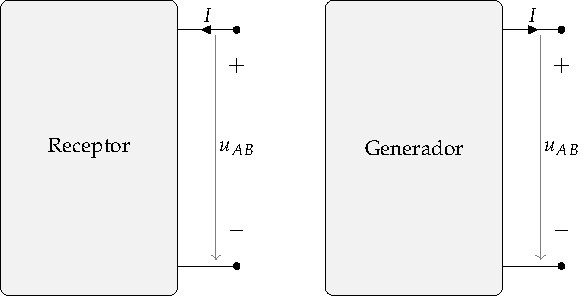
\includegraphics[height=0.5\textheight]{../figs/receptor_generador.pdf}
\end{center}
\end{frame}

\begin{frame}[label={sec:orge941b08}]{Potencia y Energía}
\begin{description}
\item[{Energía}] es la capacidad para realizar un trabajo.

Unidades Wh, kWh

1 kWh = 3.6 MJ

\item[{Potencia}] es la cantidad de trabajo efectuado \emph{por unidad de
tiempo}.

Unidades W, kW
\end{description}
\end{frame}

\begin{frame}[label={sec:org2d43c5c}]{Rendimiento/Eficiencia}
Cuadripolo (entrada/salida)
\begin{equation*}
  \eta = \frac{P_{salida}}{P_{entrada}}
\end{equation*}

Receptor
\begin{equation*}
  \eta_m = \frac{P_{util}}{P_{absorbida}}
\end{equation*}

Generador
\begin{equation*}
  \eta_g = \frac{P_{entregada}}{P_{producida}}
\end{equation*}

Cualquier máquina tiene pérdidas:

\begin{equation*}
  \boxed{\eta < 1}
\end{equation*}
\end{frame}

\begin{frame}[label={sec:org3aaebe5}]{Corriente Continua y Corriente Alterna}
\begin{itemize}
\item Corriente Continua (\(\frac{d}{dt} = 0\))
\end{itemize}
\begin{center}
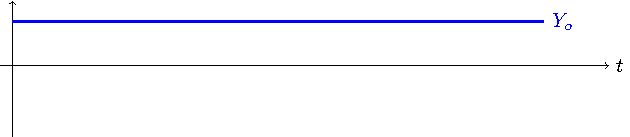
\includegraphics[width=\textwidth]{../figs/continua.pdf}
\end{center}

\begin{itemize}
\item Corriente Alterna (\(\frac{d}{dt} \neq 0\))
\end{itemize}
\begin{center}
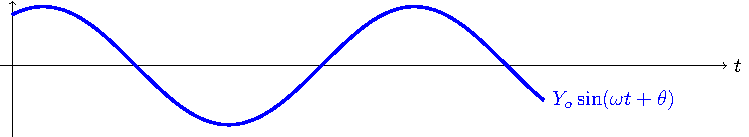
\includegraphics[width=\textwidth]{../figs/sin.pdf}
\end{center}
\end{frame}

\section{Elementos circuitales}
\label{sec:orgc7d0d3a}

\subsection{Elementos Pasivos Lineales}
\label{sec:orgd10d99d}
\begin{frame}[label={sec:org31eafd2}]{Resistencia}
\begin{itemize}
\item \alert{Ley de Ohm}: una resistencia provoca una \alert{diferencia de potencial} entre sus terminales \alert{directamente proporcional} a su corriente: \alert{resistencia} (Ohmios, [\(\Omega\)])
\end{itemize}
\[
u(t) = R \cdot i(t)
\]
\begin{itemize}
\item \alert{Criterio de Signos}: la tensión es positiva en el terminal por el que entra la corriente (las flechas de tensión y corriente tienen el mismo sentido).
\end{itemize}
\begin{columns}
\begin{column}{0.5\columnwidth}
\begin{center}
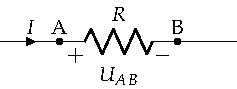
\includegraphics[height=0.2\textheight]{../figs/Resistencia.pdf}
\end{center}
\end{column}
\begin{column}{0.5\columnwidth}
\begin{center}
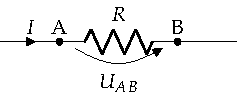
\includegraphics[height=0.2\textheight]{../figs/Resistencia_Flecha.pdf}
\end{center}
\end{column}
\end{columns}
\end{frame}

\begin{frame}[label={sec:org80e5ad5}]{Resistividad}
\begin{itemize}
\item El valor de la resistencia depende de la \alert{resistividad del material} (\(\rho\)), de la \alert{sección} (\(S\)), y de la
longitud (\(l\)):
\end{itemize}
\begin{equation*}
  R = \rho \cdot \frac{l}{S}
\end{equation*}

\begin{itemize}
\item La \alert{sección} se expresa en \(\si{\milli\meter\squared}\).

\item La \alert{resistividad} depende del material conductor y de la temperatura ambiente:

\begin{itemize}
\item Cobre a 20ºC: \(\SI{17.24}{\milli\ohm\milli\meter\squared\per\meter}\).
\end{itemize}
\end{itemize}
\end{frame}

\begin{frame}[label={sec:org2a9a652}]{Cortocircuito y Circuito Abierto}
\begin{itemize}
\item Cortocircuito: resistencia nula (tensión nula)
\end{itemize}

\begin{center}
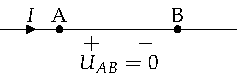
\includegraphics[height=0.2\textheight]{../figs/Cortocircuito.pdf}
\end{center}

\begin{itemize}
\item Circuito abierto: resistencia infinita (corriente nula).
\end{itemize}

\begin{center}
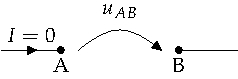
\includegraphics[height=0.2\textheight]{../figs/CircuitoAbierto.pdf}
\end{center}
\end{frame}

\begin{frame}[label={sec:org7a807b7}]{Ley de Joule}
\begin{center}
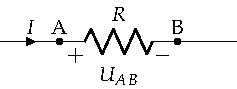
\includegraphics[height=0.2\textheight]{../figs/Resistencia.pdf}
\end{center}

\begin{itemize}
\item \alert{Ley de Joule}: una resistencia disipa energía eléctrica produciendo \alert{calor}.
\end{itemize}
\[
p(t)=R\cdot i^{2}(t)
\]
\end{frame}


\begin{frame}[label={sec:org066614b}]{Bobina o inductancia}
\begin{center}
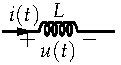
\includegraphics[height=0.2\textheight]{../figs/Bobina.pdf}
\end{center}

\begin{itemize}
\item Cuando una corriente oscilante atraviesa un conductor arrollado alrededor de un núcleo, se produce una \alert{tensión inducida que se opone a esta corriente} (ley de Faraday y Lenz)

\item La tensión en sus terminales es directamente proporcional al cambio de la corriente: coeficiente de autoinducción o \alert{inductancia} (Henrios [H]).
\end{itemize}

\[
u_L(t)=L\cdot\frac{di(t)}{dt}
\]
\end{frame}

\begin{frame}[label={sec:org83747d5}]{Bobina o inductancia}
\begin{center}
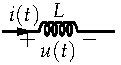
\includegraphics[height=0.2\textheight]{../figs/Bobina.pdf}
\end{center}

\begin{itemize}
\item Almacena \alert{energía magnética}.
\end{itemize}

\[
  E_L(t) = \int_{-\infty}^t u(\tau) \cdot i(\tau) d\tau = \frac{1}{2} \cdot L \cdot i^2(t)
\]
\begin{itemize}
\item En circuitos de corriente continua es un cortocircuito.
\end{itemize}

\begin{equation*}
  \frac{di(t)}{dt} = 0 \Rightarrow U_L = 0
\end{equation*}
\end{frame}

\begin{frame}[label={sec:org51868ef}]{Condensador}
\begin{center}
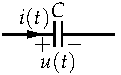
\includegraphics[height=0.2\textheight]{../figs/Condensador.pdf}
\end{center}

\begin{itemize}
\item Un \alert{condensador} está formado por dos placas metálicas separadas por una capa dieléctrica. Al aplicar tensión se produce una \alert{separación de cargas opuestas} que se \alert{acumulan} en cada placa.

\item La \alert{carga acumulada} en un instante es \alert{proporcional} a la \alert{diferencia de potencial} en ese instante: \alert{capacidad} (Faradios [F]).
\end{itemize}

\[
q(t) = C \cdot u(t)
\]

\begin{itemize}
\item En el proceso de carga se produce una corriente eléctrica entre las dos placas.
\end{itemize}
\[
i_C(t)=\frac{dq(t)}{d(t)}=C\frac{du(t)}{dt}
\]
\end{frame}


\begin{frame}[label={sec:org0ef5165}]{Condensador}
\begin{center}
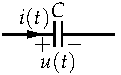
\includegraphics[height=0.2\textheight]{../figs/Condensador.pdf}
\end{center}

\begin{itemize}
\item Un condensador almacena \alert{energía eléctrica}
\end{itemize}

\[
  E_c(t) = \int_{-\infty}^t u(\tau) \cdot i(\tau) d\tau = \frac{1}{2} \cdot C \cdot u^2(t)
\]

\begin{itemize}
\item En un circuito de corriente continua se comporta como un circuito abierto.
\end{itemize}

\begin{equation*}
  \frac{du(t)}{dt} = 0 \Rightarrow I_c = 0
\end{equation*}
\end{frame}

\subsection{Elementos Pasivos No Lineales}
\label{sec:orgb309815}

\begin{frame}[label={sec:org85e483f}]{Diodo}
\begin{center}
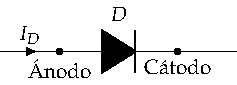
\includegraphics[height=0.15\textheight]{../figs/Diodo.pdf}
\end{center}

\begin{itemize}
\item Un diodo es un dispositivo electrónico que permite el paso de
corriente a través de él a partir de una tensión de polarización.

\item Cuando \alert{no conduce} se comporta (idealmente) como un \alert{circuito abierto}.

\item Cuando \alert{conduce} se comporta (idealmente) como un \alert{cortocircuito}.
\end{itemize}
\end{frame}

\begin{frame}[label={sec:orgf9e56a7}]{Diodo}
\begin{center}
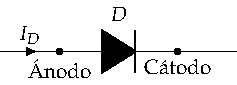
\includegraphics[height=0.15\textheight]{../figs/Diodo.pdf}
\end{center}

\begin{itemize}
\item Por tanto, puede ser utilizado como

\begin{itemize}
\item \alert{Elemento de bloqueo} (evitar que circule corriente por una parte
del circuito en ciertas condiciones)

\item \alert{Elemento de protección} (obligar a que la corriente circule por
él, evitando que circule por otra rama paralela).
\end{itemize}
\end{itemize}
\end{frame}

\begin{frame}[label={sec:org6eafd80}]{Transistor}
\begin{center}
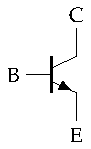
\includegraphics[height=0.3\textheight]{../figs/Transistor.pdf}
\end{center}

\begin{itemize}
\item Un transistor es un dispositivo electrónico con tres terminales que
permite el paso de corriente entre dos de sus terminales cuando en el
tercer terminal está polarizado adecuadamente.

\item Cuando \alert{no conduce} se comporta (idealmente) como un \alert{circuito abierto}.

\item Cuando \alert{conduce} se comporta (idealmente) como un \alert{cortocircuito}.
\end{itemize}
\end{frame}


\begin{frame}[label={sec:orga92e829}]{Transistor}
\begin{center}
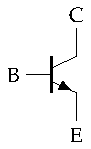
\includegraphics[height=0.3\textheight]{../figs/Transistor.pdf}
\end{center}

Por tanto, puede ser utilizado como:

\begin{itemize}
\item \alert{Elemento de conmutación} (dirigir la circulación de corriente entre
dos terminales controlando la señal en el tercer terminal)

\item \alert{Elemento de amplificación} (la señal entregada en el terminal de
control es reproducida en la salida con mayor amplitud)
\end{itemize}
\end{frame}


\subsection{Elementos Activos}
\label{sec:orga27d73d}

\begin{frame}[label={sec:org0d960db}]{Generadores de Tensión y Corriente}
\begin{columns}
\begin{column}{0.5\columnwidth}
\begin{center}
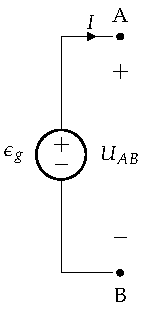
\includegraphics[height=0.5\textheight]{../figs/FuenteTensionIdealDC.pdf}
\end{center}
Un \alert{generador de tensión ideal} impone la tensión a la salida (\emph{la corriente depende del circuito}). Se caracteriza por su \alert{fuerza electromotriz} (voltios [V]).
\end{column}

\begin{column}{0.5\columnwidth}
\begin{center}
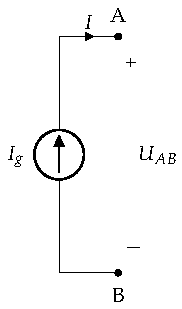
\includegraphics[height=0.5\textheight]{../figs/FuenteCorrienteIdeal.pdf}
\end{center}
Un \alert{generador de corriente ideal} impone la corriente a la salida (\emph{la tensión depende del circuito}). Se caracteriza por su corriente de generador.
\end{column}
\end{columns}
\end{frame}

\begin{frame}[label={sec:org12aeae6}]{Generador Real}
Los generadores reales tienen pérdidas que se modelan con una resistencia en \alert{serie} (generador de tensión) o en \alert{paralelo} (generador de corriente)

\begin{columns}
\begin{column}{0.5\columnwidth}
\begin{center}
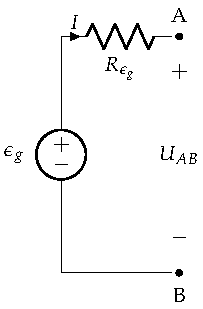
\includegraphics[height=0.7\textheight]{../figs/FuenteTensionRealDC.pdf}
\end{center}
\end{column}
\begin{column}{0.5\columnwidth}
\begin{center}
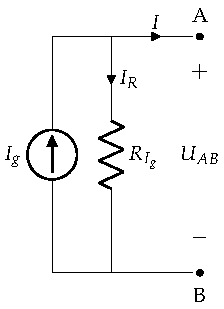
\includegraphics[height=0.7\textheight]{../figs/FuenteCorrienteRealDC.pdf}
\end{center}
\end{column}
\end{columns}
\end{frame}


\section{Leyes de Kirchhoff}
\label{sec:org02fac44}

\subsection{Definiciones}
\label{sec:org7e496fb}
\begin{frame}[label={sec:org8d05324}]{Ley de Kirchhoff de las Corrientes (LKC)}
\begin{itemize}
\item La \alert{LKC} es el principio de conservación de la carga aplicado a los circuitos eléctricos.

\item \alert{LKC}: la suma de las corrientes que llegan a un nudo es igual a la suma de las que salen.

\begin{itemize}
\item Las lineas de corriente son cerradas (o solenoidales).
\end{itemize}
\end{itemize}

\begin{center}
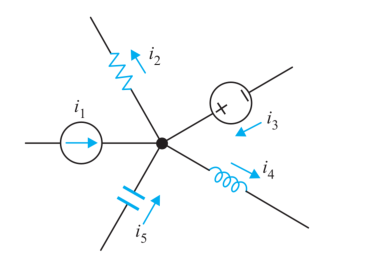
\includegraphics[height=0.4\textheight]{../figs/LKC_FM.pdf}
\end{center}
\[
i_1(t) - i_2(t) + i_3(t) - i_4(t) + i_5(t) = 0
\]
\end{frame}

\begin{frame}[label={sec:org59e4ba5}]{Ley de Kirchhoff de los Voltajes (LKV)}
\begin{itemize}
\item La \alert{LKV} es el principio de conservación de la energía aplicado a los circuitos eléctricos.

\item \alert{LKV}: la suma (con signo) de las tensiones a lo largo de un camino cerrado (circuito) es cero.

\begin{itemize}
\item La energía producida por un generador es consumida por los receptores del circuito para producir trabajo (mecánico, químico, etc.) o calor.
\end{itemize}
\end{itemize}

\begin{center}
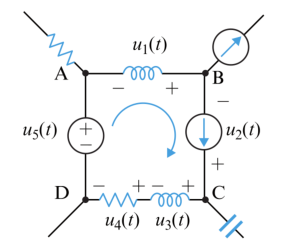
\includegraphics[height=0.4\textheight]{../figs/LKV_FM.pdf}
\end{center}
\[
u_3(t) + u_4 (t) - u_5 (t) - u_1 (t) - u_2 (t)  = 0
\]
\end{frame}

\begin{frame}[label={sec:orgbca918d}]{Balance de Tensiones}
\begin{center}
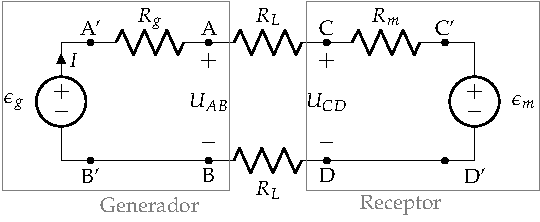
\includegraphics[width=.9\linewidth]{../figs/circuito_lkv.pdf}
\end{center}
\begin{equation*}
  U_{A'A} + U_{AC} + U_{CC'} + U_{C'D'} + U_{D'D} + U_{DB} + U_{BB'} + U_{B'A'} = 0
\end{equation*}

\begin{equation*}
  U_{AB} = U_{AA'} + U_{A'B'} + U_{B'B}
\end{equation*}

\begin{equation*}
  U_{CD} = U_{CC'} + U_{C'D'} + U_{DD'}
\end{equation*}
\end{frame}

\begin{frame}[label={sec:orgd7cd151}]{Balance de Tensiones}
\begin{center}
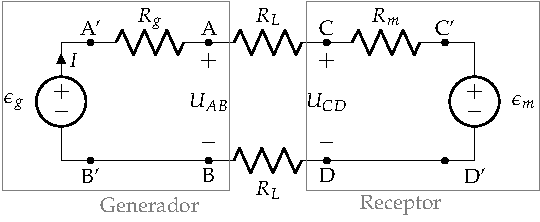
\includegraphics[height=0.3\textheight]{../figs/circuito_lkv.pdf}
\end{center}
\begin{equation*}
  U_{A'A} + U_{AC} + U_{CC'} + U_{C'D'} + U_{D'D} + U_{DB} + U_{BB'} + U_{B'A'} = 0
\end{equation*}

\begin{columns}
\begin{column}{0.3\columnwidth}
\begin{align*}
  U_{A'A} &= I \cdot R_g\\
  U_{AC} &= I \cdot R_L\\
  U_{CC'} &= I \cdot R_m\\
  U_{C'D'} &= \epsilon_m\\
  U_{D'D} &= 0 = U_{BB'}\\
  U_{DB} &= I \cdot R_L\\
  U_{B'A'} &= -\epsilon_g
\end{align*}
\end{column}
\begin{column}{0.7\columnwidth}
\begin{equation*}
  I \cdot (R_g + 2\cdot R_L + R_m) + \epsilon_m = \epsilon_g
\end{equation*}

\begin{equation*}
  U_{AB} = \epsilon_g - I \cdot R_g
\end{equation*}

\begin{equation*}
  U_{CD} = I\cdot R_m + \epsilon_m
\end{equation*}
\end{column}
\end{columns}
\end{frame}
\subsection{Asociación de Elementos}
\label{sec:org3755d78}

\begin{frame}[label={sec:org375a167}]{Conexión en serie}
\begin{columns}
\begin{column}{0.3\columnwidth}
\begin{center}
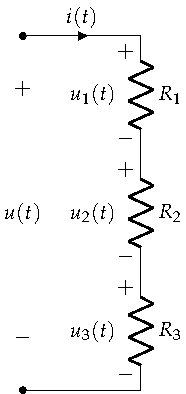
\includegraphics[width=.9\linewidth]{../figs/AsociacionSerie.pdf}
\end{center}
\end{column}
\begin{column}{0.7\columnwidth}
Un conjunto de elementos están asociados en serie cuando circula la misma corriente por todos ellos.
\begin{align*}
  u_1(t) &= R_1 \cdot i(t)\\
  u_2(t) &= R_2 \cdot i(t)\\
  u_3(t) &= R_3 \cdot i(t)
\end{align*}
\end{column}
\end{columns}
\end{frame}
\begin{frame}[label={sec:org32decf0}]{Conexión en serie}
\begin{columns}
\begin{column}{0.3\columnwidth}
\begin{center}
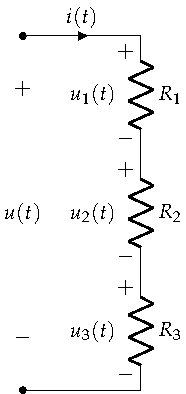
\includegraphics[width=.9\linewidth]{../figs/AsociacionSerie.pdf}
\end{center}
\end{column}
\begin{column}{0.7\columnwidth}
Aplicando LKV:
\begin{equation*}
  u(t) = u_1(t) + u_2(t) + u_3(t)
\end{equation*}

Sacando \(i(t)\) como factor común:
\begin{equation*}
  u(t) = i(t) \cdot (R_1 + R_2 + R_3)
\end{equation*}

Definimos la resistencia equivalente de la conexión serie:
\begin{align*}
  \Aboxed{R_s &= \sum_{i = 1}^n R_i}\\
  u(t) &= R_s \cdot i(t)
\end{align*}
\end{column}
\end{columns}
\end{frame}

\begin{frame}[label={sec:org98b2ab8}]{Conexión en serie de inductancias}
\begin{columns}
\begin{column}{0.3\columnwidth}
\begin{center}
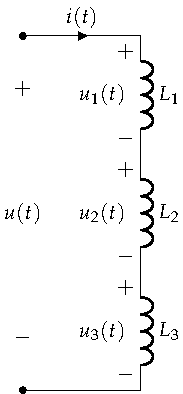
\includegraphics[width=.9\linewidth]{../figs/BobinasSerie.pdf}
\end{center}
\end{column}
\begin{column}{0.7\columnwidth}
\begin{align*}
  u_1(t) &= L_1 \cdot \frac{di(t)}{dt}\\
  u_2(t) &= L_2 \cdot \frac{di(t)}{dt}\\
  u_3(t) &= L_3 \cdot \frac{di(t)}{dt}\\
\end{align*}

\begin{align*}
  \Aboxed{L_s &= \sum_{i = 1}^n L_i}\\
  u(t) &= L_s \cdot \frac{di(t)}{dt}
\end{align*}
\end{column}
\end{columns}
\end{frame}

\begin{frame}[label={sec:orgf619ad8}]{Conexión en serie de condensadores}
\begin{columns}
\begin{column}{0.3\columnwidth}
\begin{center}
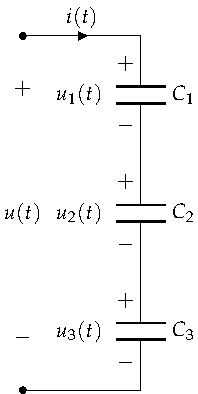
\includegraphics[width=.9\linewidth]{../figs/CondensadoresSerie.pdf}
\end{center}
\end{column}
\begin{column}{0.7\columnwidth}
\begin{align*}
  i(t) &= C_1 \cdot \frac{du_1(t)}{dt}\\
  i(t) &= C_2 \cdot \frac{du_2(t)}{dt}\\
  i(t) &= C_3 \cdot \frac{du_3(t)}{dt}\\
\end{align*}

\begin{align*}
  \Aboxed{\frac{1}{C_s} &= \sum_{i = 1}^n \frac{1}{C_i}}\\
  i(t) &= C_s \cdot \frac{du(t)}{dt}
\end{align*}
\end{column}
\end{columns}
\end{frame}

\begin{frame}[label={sec:org4f69d6d}]{Conexión en paralelo}
Un conjunto de elementos están asociados en paralelo cuando están sometidos a la misma diferencia de potencial.
\begin{center}
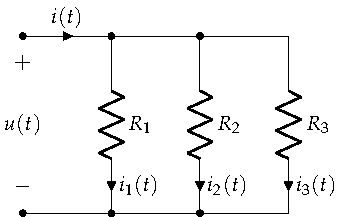
\includegraphics[height=0.45\textheight]{../figs/AsociacionParalelo.pdf}
\end{center}

\begin{align*}
  i_1(t) &= u(t)/R_1\\
  i_2(t) &= u(t)/R_2\\
  i_3(t) &= u(t)/R_3
\end{align*}
\end{frame}
\begin{frame}[label={sec:org5b86664}]{Conexión en paralelo}
\begin{columns}
\begin{column}{0.4\columnwidth}
\begin{center}
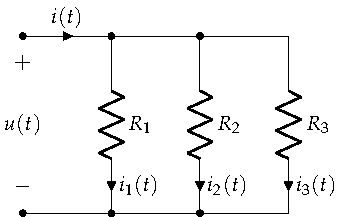
\includegraphics[width=.9\linewidth]{../figs/AsociacionParalelo.pdf}
\end{center}
\end{column}
\begin{column}{0.6\columnwidth}
Aplicando LKC:
\begin{equation*}
  i(t) = i_1(t) + i_2(t) + i_3(t)
\end{equation*}

Sacando \(u(t)\) como factor común:
\begin{equation*}
  i(t) = u(t) \cdot (\frac{1}{R_1} + \frac{1}{R_2} + \frac{1}{R_3})
\end{equation*}

Definimos la resistencia equivalente de la conexión paralelo:
\begin{align*}
  \Aboxed{\frac{1}{R_p} &= \sum_{i = 1}^n \frac{1}{R_i}}\\
  u(t) &= R_p \cdot i(t)
\end{align*}
\end{column}
\end{columns}
\end{frame}
\begin{frame}[label={sec:orgdeed21f}]{Dos resistencias en paralelo}
En el caso concreto de \alert{dos} resistencias en paralelo \ldots{}
\begin{equation*}
  \frac{1}{R_p} = \frac{1}{R_1} + \frac{1}{R_2}
\end{equation*}
\ldots{} la expresión es:
\begin{equation*}
  \boxed{R_p = \frac{R_1 \cdot R_2}{R_1 + R_2}}
\end{equation*}
\end{frame}

\begin{frame}[label={sec:org749a8c7}]{Conexión en paralelo de inductancias}
\begin{center}
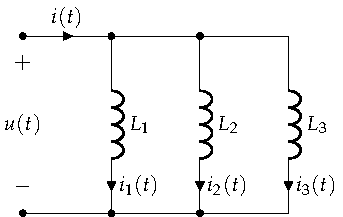
\includegraphics[height=0.45\textheight]{../figs/BobinasParalelo.pdf}
\end{center}

\begin{columns}
\begin{column}{0.5\columnwidth}
\begin{align*}
  u(t) &= L_1 \cdot \frac{di_1(t)}{dt}\\
  u(t) &= L_2 \cdot \frac{di_2(t)}{dt}\\
  u(t) &= L_3 \cdot \frac{di_3(t)}{dt}\\
\end{align*}
\end{column}
\begin{column}{0.5\columnwidth}
\begin{align*}
  \Aboxed{\frac{1}{L_p} &= \sum_{i = 1}^n \frac{1}{L_i}}\\
  u(t) &= L_p \cdot \frac{di(t)}{dt}
\end{align*}
\end{column}
\end{columns}
\end{frame}

\begin{frame}[label={sec:orgf1406e3}]{Conexión en paralelo de condensadores}
\begin{center}
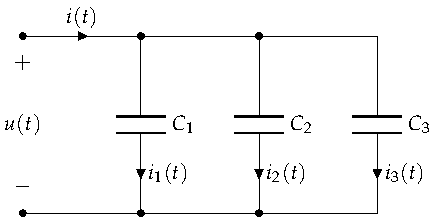
\includegraphics[height=0.45\textheight]{../figs/CondensadoresParalelo.pdf}
\end{center}
\begin{columns}
\begin{column}{0.5\columnwidth}
\begin{align*}
  i_1(t) &= C_1 \cdot \frac{du(t)}{dt}\\
  i_2(t) &= C_2 \cdot \frac{du(t)}{dt}\\
  i_3(t) &= C_3 \cdot \frac{du(t)}{dt}\\
\end{align*}
\end{column}
\begin{column}{0.5\columnwidth}
\begin{align*}
  \Aboxed{C_p &= \sum_{i = 1}^n C_i}\\
  i(t) &= C_p \cdot \frac{du(t)}{dt}
\end{align*}
\end{column}
\end{columns}
\end{frame}
\section{Corriente Alterna Sinusoidal}
\label{sec:org1a17dbb}
\subsection{Conceptos Fundamentales}
\label{sec:orgf7b7131}
\begin{frame}[label={sec:orgf1619a3}]{Onda sinusoidal}
\begin{center}
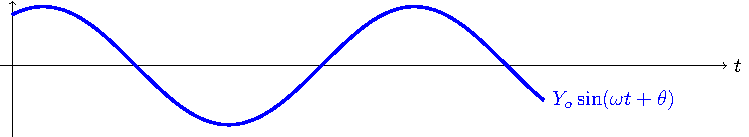
\includegraphics[width=.9\linewidth]{../figs/sin.pdf}
\end{center}


\[
y(t)=Y_{o}\cdot\sin(\omega\cdot t+\theta)
\]

\begin{itemize}
\item \(Y_{o}\) valor máximo de la onda.

\item \(\omega=\frac{2\cdot\pi}{T}\): pulsación (radianes/segundo)

\item T: periodo de la onda (segundos)

\item \(f=\frac{\omega}{2\cdot\pi}=\frac{1}{T}\): frecuencia (Hz)
\end{itemize}
\end{frame}


\begin{frame}[label={sec:org06e8294}]{Fase}
\begin{center}
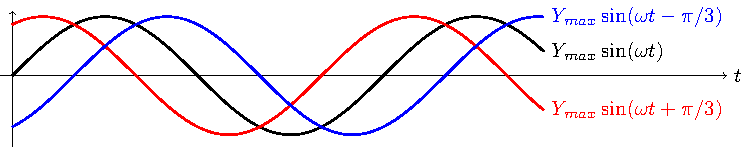
\includegraphics[width=.9\linewidth]{../figs/desfase.pdf}
\end{center}


\[
y(t)=Y_{o}\cdot\sin(\omega\cdot t+\theta)
\]

\begin{itemize}
\item \(\theta\): fase (radianes o grados)

\begin{itemize}
\item Es el argumento de la onda para t=0

\item Tomando una onda como referencia, si la fase es 0º, se dice que
están en fase con la onda de referencia.

\item Si la fase es positiva, se dice que la onda adelanta
respecto a la referencia.
\end{itemize}
\end{itemize}
\end{frame}


\begin{frame}[label={sec:org326fefb}]{Señales en Cuadratura}
\begin{center}
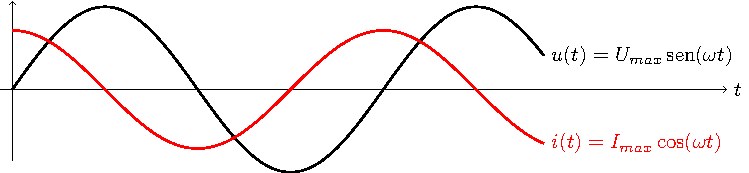
\includegraphics[width=.9\linewidth]{../figs/cuadratura.pdf}
\end{center}

\begin{itemize}
\item Cuando el desfase entre dos señales es de 90º (\(\theta_I - \theta_U = \pi/2\)), se dice que están en cuadratura.
\item El paso por cero de una señal coincide con el paso por el máximo/mínimo de la otra señal.
\end{itemize}
\end{frame}


\begin{frame}[label={sec:orgc8170f7}]{Valor medio y valor eficaz}
\begin{block}{Valor medio}
\[
Y_m=\frac{1}{T}\int_{0}^{T}y(t)\, dt
\]

\[
Y_m=\frac{1}{T}\int_{0}^{T}Y_{o}\cdot\sin(\omega\cdot+\theta)\, dt=0
\]
\end{block}
\begin{block}{Valor eficaz}
\[
Y = \sqrt{\frac{1}{T}\cdot\int_{0}^{T}y^{2}(t)\, dt}
\]

\[
Y=\sqrt{\frac{1}{T}\cdot\int_{0}^{T}\left(Y_{o}\cdot\sin(\omega\cdot t+\theta)\right)^{2}dt}=\boxed{\frac{Y_{o}}{\sqrt{2}}}
\]
\end{block}
\end{frame}

\subsection{Cálculo Fasorial}
\label{sec:orga3886a8}

\begin{frame}[label={sec:org94de950}]{Representación fasorial}
\begin{itemize}
\item Un fasor es un \alert{número complejo} que representa una señal sinusoidal para simplificar cálculos.
\item El \alert{módulo} del fasor es el \alert{valor eficaz}. El \alert{argumento} es la \alert{fase}.
\item Descartamos pulsación: No se puede emplear cuando hay frecuencias diferentes en un mismo circuito.
\end{itemize}

\begin{columns}
\begin{column}{0.5\columnwidth}
\begin{align*}
\overline{Y} &= Y\cdot e^{j\theta}\\
\overline{Y} &= Y\phase{\theta}\\
\overline{Y} &= Y\cdot(\cos(\theta)+\mathrm{j}\cdot\sin(\theta))
\end{align*}
\end{column}

\begin{column}{0.5\columnwidth}
\begin{center}
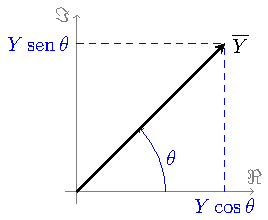
\includegraphics[height=0.45\textheight]{../figs/fasor.pdf}
\end{center}
\end{column}
\end{columns}
\end{frame}

\begin{frame}[label={sec:org262bf15}]{Tensión y corriente en notación fasorial}
\begin{center}
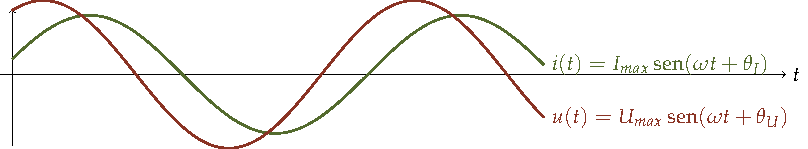
\includegraphics[width=.9\linewidth]{../figs/ondasTensionCorriente.pdf}
\end{center}

\begin{columns}
\begin{column}{0.5\columnwidth}
\begin{align*}
  \overline{U} &= U\phase{\theta_U}\\
  \overline{I} &= I\phase{\theta_I}
\end{align*}
\end{column}

\begin{column}{0.5\columnwidth}
\begin{center}
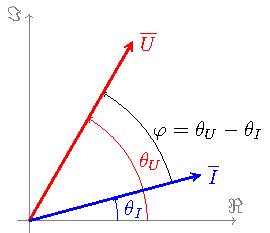
\includegraphics[height=0.5\textheight]{../figs/fasorTensionCorriente.pdf}
\end{center}
\end{column}
\end{columns}
\end{frame}


\begin{frame}[label={sec:org107c8b4}]{Impedancia: relación entre fasores de tensión y corriente}
\begin{columns}
\begin{column}{0.5\columnwidth}
\begin{align*}
  \overline{U} &= \overline{Z} \cdot \overline{I}\\                 
  \overline{Z} &= \frac{\overline{U}}{\overline{I}}
\end{align*}

\[
\boxed{\overline{Z} = \frac{U}{I}\phase{\theta_U - \theta_I} \Rightarrow 
    \begin{cases}
      Z = \frac{U}{I}\\
      \theta = \theta_U - \theta_I
    \end{cases}}
\]
\end{column}


\begin{column}{0.5\columnwidth}
\begin{center}
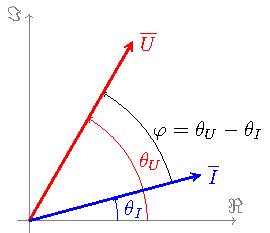
\includegraphics[height=0.5\textheight]{../figs/fasorTensionCorriente.pdf}
\end{center}
\end{column}
\end{columns}
\end{frame}


\begin{frame}[label={sec:org810bd41}]{Impedancia Genérica}
\[
\overline{Z} = R + j X
\]

\begin{center}
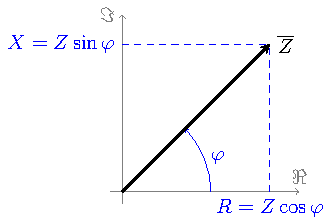
\includegraphics[width=.9\linewidth]{../figs/fasorImpedancia.pdf}
\end{center}
\end{frame}


\begin{frame}[label={sec:org6936797}]{Circuito Resistivo}
Un circuito resistivo no desfasa (\alert{tensión y corriente en fase}).

\begin{center}
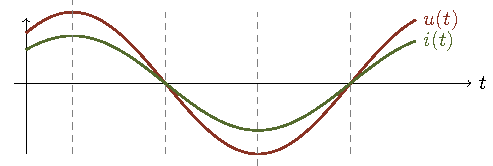
\includegraphics[width=.9\linewidth]{../figs/resistivo.pdf}
\end{center}

\begin{columns}
\begin{column}{0.3\columnwidth}
\[
\overline{Z}_R = R = R \phase{0}
\]
\end{column}

\begin{column}{0.35\columnwidth}
\begin{center}
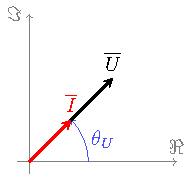
\includegraphics[width=.9\linewidth]{../figs/fasorResistencia_VI.pdf}
\end{center}
\end{column}


\begin{column}{0.35\columnwidth}
\begin{center}
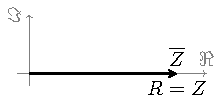
\includegraphics[width=.9\linewidth]{../figs/fasorResistencia.pdf}
\end{center}
\end{column}
\end{columns}
\end{frame}





\begin{frame}[label={sec:org34ec9b8}]{Circuito Inductivo puro}
Un circuito inductivo puro genera \alert{señales en cuadratura} y \alert{retrasa la corriente}.

\begin{center}
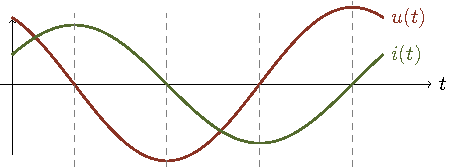
\includegraphics[height=0.3\textheight]{../figs/inductivoPuro.pdf}
\end{center}

\begin{columns}
\begin{column}{0.3\columnwidth}
\[
\overline{Z}_L = j\omega L = \omega L \phase{\ang{90}}
\]
\end{column}


\begin{column}{0.4\columnwidth}
\begin{center}
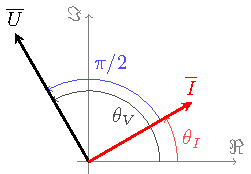
\includegraphics[width=.9\linewidth]{../figs/fasorInductancia_VI.pdf}
\end{center}
\end{column}


\begin{column}{0.3\columnwidth}
\begin{center}
\includegraphics[height=0.4\textheight]{../figs/fasorInductancia.pdf}
\end{center}
\end{column}
\end{columns}
\end{frame}



\begin{frame}[label={sec:org3de4ee3}]{Circuito Capacitivo puro}
Un circuito capacitivo puro genera \alert{señales en cuadratura} y \alert{adelanta la corriente}.

\begin{center}
\includegraphics[height=0.3\textheight]{../figs/capacitivoPuro.pdf}
\end{center}

\begin{columns}
\begin{column}{0.3\columnwidth}
\[
\overline{Z}_C = \frac{1}{j\omega C} = \frac{1}{\omega C}\phase{\ang{-90}}
\]
\end{column}


\begin{column}{0.4\columnwidth}
\begin{center}
\includegraphics[width=.9\linewidth]{../figs/fasorCondensador_VI.pdf}
\end{center}
\end{column}


\begin{column}{0.3\columnwidth}
\begin{center}
\includegraphics[height=0.4\textheight]{../figs/fasorCondensador.pdf}
\end{center}
\end{column}
\end{columns}
\end{frame}

\begin{frame}[label={sec:org94c231d}]{Circuito RL (inductivo con pérdidas)}
\begin{center}
\includegraphics[height=0.25\textheight]{../figs/inductivo.pdf}
\end{center}
\begin{columns}
\begin{column}{0.45\columnwidth}
\begin{center}
\includegraphics[width=.9\linewidth]{../figs/RL.pdf}
\end{center}

\begin{align*}
  \overline{U} &= \overline{U}_R + \overline{U}_L =\\
	       &=(R + j\omega L) \overline{I}
\end{align*}
\end{column}
\begin{column}{0.55\columnwidth}
\begin{center}
\includegraphics[height=0.5\textheight]{../figs/fasorInductanciaReal_VI.pdf}
\end{center}
\end{column}
\end{columns}
\end{frame}

\begin{frame}[label={sec:org0eb4a0b}]{Circuito RL (inductivo con pérdidas)}
\begin{center}
\includegraphics[height=0.2\textheight]{../figs/RL.pdf}
\end{center}

\begin{columns}
\begin{column}{0.45\columnwidth}
\[
\overline{Z} = R + j\omega L \Rightarrow \boxed{\theta > 0}
\]
\[
  |Z| = \sqrt{R^2 + (\omega L)^2}
\]
\[
  \theta = \atan{\frac{\omega L}{R}}
\]
\end{column}

\begin{column}{0.55\columnwidth}
\begin{center}
\includegraphics[width=.9\linewidth]{../figs/fasorInductanciaReal.pdf}
\end{center}
\end{column}
\end{columns}
\end{frame}


\begin{frame}[label={sec:org96560ee}]{Circuito RC (capacitivo con pérdidas)}
\begin{center}
\includegraphics[height=0.25\textheight]{../figs/capacitivo.pdf}
\end{center}


\begin{columns}
\begin{column}{0.45\columnwidth}
\begin{center}
\includegraphics[width=.9\linewidth]{../figs/RC.pdf}
\end{center}

\begin{align*}
  \overline{U} &= \overline{U}_R + \overline{U}_C =\\
               &= (R - j \frac{1}{\omega C}) \overline{I} 
\end{align*}
\end{column}
\begin{column}{0.55\columnwidth}
\begin{center}
\includegraphics[height=0.45\textheight]{../figs/fasorCondensadorReal_VI.pdf}
\end{center}
\end{column}
\end{columns}
\end{frame}


\begin{frame}[label={sec:org3174818}]{Circuito RC (capacitivo con pérdidas)}
\begin{center}
\includegraphics[height=0.2\textheight]{../figs/RC.pdf}
\end{center}

\begin{columns}
\begin{column}{0.45\columnwidth}
\[
\overline{Z} = R - \frac{j}{\omega C} \Rightarrow \boxed{\theta < 0}
\]

\[
  |Z| = \sqrt{R^2 + \frac{1}{(\omega C)^2}}
\]

\[
  \theta = - \atan{\frac{1}{\omega R C}}
\]
\end{column}

\begin{column}{0.55\columnwidth}
\begin{center}
\includegraphics[height=0.45\textheight]{../figs/fasorCondensadorReal.pdf}
\end{center}
\end{column}
\end{columns}
\end{frame}


\begin{frame}[label={sec:org368dd76}]{Circuito RLC serie}
\begin{center}
\includegraphics[height=0.2\textheight]{../figs/RLC.pdf}
\end{center}

\begin{columns}
\begin{column}{0.4\columnwidth}
\[
\overline{Z} = R + j(\omega L - \frac{1}{\omega C})
\]
\[
  |Z| = \sqrt{R^2 + (\omega L - \frac{1}{\omega C})^2}
\]
\[
  \theta = \atan{\frac{\omega L - \frac{1}{\omega C}}{R}}
\]
\end{column}

\begin{column}{0.6\columnwidth}
\begin{itemize}
\item \(\theta > 0 \Rightarrow \omega L > \frac{1}{\omega C}\): inductivo
\item \(\theta < 0 \Rightarrow \omega L < \frac{1}{\omega C}\): capacitivo
\item \(\theta = 0 \Rightarrow \omega L = \frac{1}{\omega C}\): resistivo (resonancia)
\end{itemize}
\end{column}
\end{columns}

\[
\boxed{u(t) = Z \cdot I_o \sin(\omega t + \theta_I + \theta)}
\]
\end{frame}

\subsection{Potencia}
\label{sec:org4b6fd72}
\begin{frame}[label={sec:orgff72bde}]{Circuito Resistivo}
\begin{center}
\includegraphics[width=.9\linewidth]{../figs/resistivoPotencia.pdf}
\end{center}

\begin{itemize}
\item Fluctúa al doble de frecuencia.
\item Es siempre positiva.
\end{itemize}
\end{frame}

\begin{frame}[label={sec:org39f8a79}]{Circuito Inductivo puro}
\begin{center}
\includegraphics[width=.9\linewidth]{../figs/inductivoPuroPotencia.pdf}
\end{center}

\begin{itemize}
\item Fluctúa al doble de frecuencia.
\item Pasa por los ceros de tensión y corriente.
\item Su valor medio es nulo.
\end{itemize}
\end{frame}

\begin{frame}[label={sec:org2dbc6e1}]{Circuito Capacitivo puro}
\begin{center}
\includegraphics[width=.9\linewidth]{../figs/capacitivoPuroPotencia.pdf}
\end{center}

\begin{itemize}
\item Fluctúa al doble de frecuencia.
\item Pasa por los ceros de tensión y corriente.
\item Su valor medio es nulo.
\end{itemize}
\end{frame}

\begin{frame}[label={sec:orgd3fb18b}]{Circuito Inductivo con pérdidas}
\begin{center}
\includegraphics[width=.9\linewidth]{../figs/inductivoPotencia.pdf}
\end{center}

\begin{center}
Valor medio positivo, \(P = U I \cos \theta\)
\end{center}
\end{frame}


\begin{frame}[label={sec:orge8736f3}]{Circuito Capacitivo con pérdidas}
\begin{center}
\includegraphics[width=.9\linewidth]{../figs/capacitivoPotencia.pdf}
\end{center}

\begin{center}
Valor medio positivo, \(P = U I \cos \theta\)
\end{center}
\end{frame}

\begin{frame}[label={sec:orge2a7f60}]{Triángulo de Potencias}
\begin{columns}
\begin{column}{0.4\columnwidth}
\begin{itemize}
\item Potencia Activa [\(W\)]
\end{itemize}
\[  
\boxed{P = U\cdot I\cdot\cos(\theta) = R \cdot I^2}
\]

\begin{itemize}
\item Potencia Reactiva [\(var\)]
\end{itemize}
\[
\boxed{Q = U\cdot I\cdot\sin(\theta) = X \cdot I^2}
\]

\begin{itemize}
\item Potencia Aparente [\(VA\)]
\end{itemize}
\[
\boxed{\overline{S} = P + jQ = \overline{U} \cdot \overline{I}^*}
\]
\end{column}

\begin{column}{0.6\columnwidth}
\begin{center}
\includegraphics[width=.9\linewidth]{/home/oscar/github/figs/trianguloPotencias.pdf}
\end{center}

\[
|S| = U \cdot I
\]
\[
\theta_S = \theta_Z = \theta
\]
\[
f.d.p. \equiv \cos(\theta)
\]
\end{column}
\end{columns}
\end{frame}
\begin{frame}[label={sec:org5a6edb8}]{Potencia de elementos: Resistencia}
\[
\theta = 0 \Rightarrow 
\begin{cases}
  P_R = R I^2\\
  Q_R = 0\\
  S_R = P_R
\end{cases}
\]

\begin{itemize}
\item Consume potencia activa
\item No consume potencia reactiva
\end{itemize}
\end{frame}

\begin{frame}[label={sec:org21252b7}]{Potencia de elementos: Inductancia}
\[
\theta = \pi/2 \Rightarrow 
\begin{cases}
  P_L = 0\\
  Q_L = \omega L I^2\\
  \overline{S}_L = \omega L I^2 \phase{\pi/2}
\end{cases}
\]

\begin{itemize}
\item No consume potencia activa
\item Consume potencia reactiva (\(Q > 0\))
\end{itemize}
\end{frame}

\begin{frame}[label={sec:org2feb28f}]{Potencia de elementos: Condensador}
\[
\theta = - \pi/2 \Rightarrow 
\begin{cases}
  P_L = 0\\
  Q_C = - \omega C U^2\\
  \overline{S}_C = \omega C U^2 \phase{-\pi/2}
\end{cases}
\]

\begin{itemize}
\item No consume potencia activa
\item Genera potencia reactiva (\(Q < 0\))
\end{itemize}
\end{frame}

\begin{frame}[label={sec:org1aa831a}]{Teorema de Boucherot}
\begin{itemize}
\item En un circuito con múltiples elementos, la potencia aparente total es la suma de las potencias aparentes individuales.
\end{itemize}
\begin{align*}
  \overline{S} &= \sum_{i = 1}^{n} \overline{S}_i\\
  P + jQ &= \sum^n_{i = 1} (P_i + jQ_i)
\end{align*}

\begin{itemize}
\item La potencia activa (reactiva) total es la suma de las potencias activas (reactivas) individuales.
\end{itemize}

\begin{align*}
P &= \sum_{i = 1}^n P_i\\
Q &= \sum_{i = 1}^n Q_i
\end{align*}
\end{frame}

\subsection{Compensación de reactiva}
\label{sec:org43de7a0}

\begin{frame}[label={sec:org2cf088c}]{Factor de potencia}
El factor de potencia, \(\cos(\theta)\), representa la aportación de potencia activa dentro de la potencia aparente.
\[
P = S \cos \theta
\]

Sean dos sistemas con \alert{misma tensión y potencia activa}, y factores de potencia \(\cos \theta_2 < \cos \theta_1\) (\(Q_2 > Q_1\))

\begin{center}
\includegraphics[height=0.5\textheight]{../figs/Fasores_CompensacionReactiva.pdf}
\end{center}
\end{frame}

\begin{frame}[label={sec:org603bbe8}]{Potencia Aparente}
\begin{center}
\includegraphics[height=0.5\textheight]{../figs/Fasores_CompensacionReactiva.pdf}
\end{center}


El sistema 2 requiere \alert{mayor potencia aparente} (generador mayor) para alimentar la misma potencia activa.
\[
  \left(\frac{P}{\cos \theta_1} = S_1 \right) < \left( S_2 = \frac{P}{\cos \theta_2}\right) 
\]
\end{frame}

\begin{frame}[label={sec:org9d7e2ab}]{Sección de Conductores}
\begin{center}
\includegraphics[height=0.5\textheight]{../figs/Fasores_CompensacionReactiva.pdf}
\end{center}

El sistema 2 requiere \alert{mayor sección} de cable para transportar la misma potencia activa.
\[
  \left(\frac{P}{U \cos \theta_1} = I_1 \right) < \left( I_2 = \frac{P}{U \cos \theta_2}\right) 
\]
\end{frame}

\begin{frame}[label={sec:org5cc29ef}]{Generación Local de Reactiva}
\begin{itemize}
\item Comúnmente, el factor de potencia es \alert{inductivo} (máquinas eléctricas
industriales).

\item La red debe suministrar potencia reactiva inductiva (influye en secciones de líneas y tamaños de generadores)

\item Es necesario mejorar \alert{localmente} el factor de potencia. Solución
común: utilizar \alert{bancos de condensadores} como suministradores de
potencia reactiva.
\end{itemize}
\end{frame}

\begin{frame}[label={sec:org3faf99b}]{Compensación de Reactiva con Condensadores}
Sea una carga de potencia activa \(P_z\), potencia reactiva \(Q_z\), factor de potencia \(\cos\theta\). Se desea \alert{mejorar el factor de potencia} a \(\cos \theta' > \cos \theta\).

\begin{center}
\includegraphics[height=0.4\textheight]{../figs/Circuito_CompensacionReactiva.pdf}
\end{center}

\begin{align*}
  P' &= P_z\\
  Q' &= Q_c + Q_z \quad (Q' < Q_z)\\
  \overline{I}' &= \overline{I}_c + \overline{I_z} \quad (I' < I_z)\\
\end{align*}
\end{frame}

\begin{frame}[label={sec:orgb201faa}]{Cálculo de la Capacidad}
\begin{center}
\includegraphics[height=0.3\textheight]{../figs/Circuito_CompensacionReactiva.pdf}
\end{center}

\begin{align*}
Q_z &= P_z \tan \theta\\
Q'&= P_z \tan \theta'\\
|Q_c| &= Q_z - Q' = P_z (\tan \theta - \tan \theta')
\end{align*}
\[
|Q_c| = \omega C U^2 \rightarrow \boxed{C = \frac{P_z (\tan \theta - \tan \theta')}{\omega U^2}}
\]
\end{frame}




\section{Corriente Alterna Trifásica}
\label{sec:org09a3be1}
\subsection{Introducción}
\label{sec:org087c2b3}
\begin{frame}[label={sec:org630c2e4}]{Motivación de los sistemas trifásicos}
\begin{itemize}
\item En un sistema trifásico la potencia instantánea es constante, evitando vibraciones y esfuerzos en las máquinas. (\emph{La potencia instantánea de un sistema monofásico es pulsante.})

\item La masa de conductor necesaria en un sistema trifásico es un 25\% inferior que en un monofásico para transportar la misma potencia.
\end{itemize}
\end{frame}

\begin{frame}[label={sec:org9a68bc2}]{Ondas Trifásicas}
\begin{center}
\includegraphics[width=.9\linewidth]{../figs/TensionesTrifasica.pdf}
\end{center}

\begin{align*}
  u_1(t) &= U_0 \cos(\omega t)\\
  u_2(t) &= U_0 \cos(\omega t + 2\pi/3)\\
  u_3(t) &= U_0 \cos(\omega t - 2\pi/3)
\end{align*}
\end{frame}

\begin{frame}[label={sec:orgdeaac5f}]{Generadores}
\begin{center}
\includegraphics[height=0.5\textheight]{../figs/GeneradoresTrifasica.pdf}
\end{center}

\begin{columns}
\begin{column}{0.5\columnwidth}
\begin{align*}
  u_1(t) &= U_0 \cos(\omega t)\\
  u_2(t) &= U_0 \cos(\omega t + 2\pi/3)\\
  u_3(t) &= U_0 \cos(\omega t - 2\pi/3)
\end{align*}
\end{column}

\begin{column}{0.5\columnwidth}
\begin{align*}
  \overline{U}_1 &= U\phase{0}\\
  \overline{U}_2 &= U\phase{2\pi/3}\\
  \overline{U}_3 &= U\phase{-2\pi/3}
\end{align*}
\end{column}
\end{columns}
\end{frame}

\begin{frame}[label={sec:orgcf5752b}]{Las tensiones suman 0}
\begin{center}
\includegraphics[height=0.6\textheight]{../figs/FasoresSumaCero.pdf}
\end{center}

\[
\boxed{\overline{U}_1 + \overline{U}_2 + \overline{U}_3 = 0}
\]
\end{frame}

\begin{frame}[label={sec:org1a53ab9}]{Las tensiones suman 0}
\begin{center}
\includegraphics[width=.9\linewidth]{../figs/TensionesTrifasica.pdf}
\end{center}

\[
\boxed{u_1(t) + u_2(t) + u_3(t) = 0}
\]
\end{frame}


\begin{frame}[label={sec:org9705acc}]{Tensiones de Fase y Línea}
\begin{columns}
\begin{column}{0.5\columnwidth}
\begin{center}
\includegraphics[height=0.4\textheight]{../figs/FasoresTrifasica_ABC.pdf}
\end{center}


Tensiones de \alert{Fase}: \(U_A\), \(U_B\), \(U_C\)

Tensiones de \alert{Línea}: \(U_{AB}\), \(U_{BC}\), \(U_{CA}\)
\end{column}


\begin{column}{0.5\columnwidth}
     \begin{align*}
       \overline{U}_{AB} &= \overline{U}_A - \overline{U}_B\\
       \overline{U}_{BC} &= \overline{U}_B - \overline{U}_C\\
       \overline{U}_{CA} &= \overline{U}_C - \overline{U}_A\\
\cline{1-2}
       \overline{U}_{AB} + \overline{U}_{BC} + \overline{U}_{CA} &= 0     \end{align*}

\[
  \boxed{
    \begin{array}{l}
      U = \sqrt{3}\cdot U_f\\
      \theta_l = \theta_f + \ang{30}\\
    \end{array}
  }
\]
\end{column}
\end{columns}
\end{frame}

\begin{frame}[label={sec:org1a3b36f}]{Secuencia de Fases}
\begin{itemize}
\item Sentido en el que ocurren los máximos de cada fase.
\item Secuencia de Fases Directa (\alert{SFD}): ABC
\end{itemize}
\begin{center}
\includegraphics[height=0.3\textheight]{../figs/TensionesTrifasica_ABC.pdf}
\end{center}
\begin{itemize}
\item Secuencia de Fases Inversa (\alert{SFI}): ACB
\end{itemize}
\begin{center}
\includegraphics[height=0.3\textheight]{../figs/TensionesTrifasica_ACB.pdf}
\end{center}
\end{frame}

\subsection{Receptores}
\label{sec:orga6fffd5}
\begin{frame}[label={sec:org978c0c6}]{Tipos de Receptores}
\begin{block}{Conexión}
\begin{itemize}
\item \alert{Estrella} (punto común) Y
\item \alert{Triángulo} \(\triangle\)
\end{itemize}
\end{block}

\begin{block}{Impedancias}
\begin{itemize}
\item \alert{Equilibrado} (las tres impedancias son idénticas en módulo \alert{y} fase).
\item \alert{Desequilibrado}
\end{itemize}
\end{block}
\end{frame}


\begin{frame}[label={sec:orgf01a603}]{Receptor en Estrella Equilibrado}
\begin{center}
\includegraphics[width=.9\linewidth]{../figs/EstrellaEquilibrado.pdf}
\end{center}
\end{frame}

\begin{frame}[label={sec:org65d3717}]{Receptor en Estrella Equilibrado}
\begin{columns}
\begin{column}{0.5\columnwidth}
\begin{center}
\includegraphics[width=.9\linewidth]{../figs/EstrellaEquilibrado_Receptor.pdf}
\end{center}
\end{column}

\begin{column}{0.5\columnwidth}
\[
  \boxed{|\overline{I}_A| = |\overline{I}_B| = |\overline{I}_C| = \frac{U_f}{Z}}
\]

\[
  \overline{I}_A  + \overline{I}_B + \overline{I}_C + \overline{I}_N = 0
\]
\[
   \overline{I}_A  + \overline{I}_B + \overline{I}_C  = 0 \rightarrow \boxed{\overline{I}_N = 0}
\]
\end{column}
\end{columns}
\end{frame}
\begin{frame}[label={sec:org6c50189}]{Receptor en Estrella Equilibrado}
\begin{center}
\includegraphics[width=.9\linewidth]{../figs/EstrellaEquilibrado_SinNeutro.pdf}
\end{center}
\end{frame}

\begin{frame}[label={sec:orgbc8d5a5}]{Receptor en Triángulo Equilibrado}
\begin{center}
\includegraphics[width=.9\linewidth]{../figs/TrianguloEquilibrado.pdf}
\end{center}
\end{frame}

\begin{frame}[label={sec:orgbb89421}]{Receptor en Triángulo Equilibrado}
\begin{columns}
\begin{column}{0.5\columnwidth}
\begin{center}
\includegraphics[width=.9\linewidth]{../figs/TrianguloEquilibrado_Receptor.pdf}
\end{center}
\end{column}

\begin{column}{0.5\columnwidth}
Corriente de Fase:
\[
  \boxed{I_f = |\overline{I}_{AB}| = |\overline{I}_{BC}| = |\overline{I}_{CA}| = \frac{U}{Z}}
\]


Corriente de Línea:
\[
  \boxed{I = |\overline{I}_A| = |\overline{I}_B| = |\overline{I}_C| = \sqrt{3} \cdot \frac{U}{Z}}
\]

\[
  \boxed{I = \sqrt{3} \cdot I_f}
\]
\end{column}
\end{columns}
\end{frame}

\begin{frame}[label={sec:org1fdf8a8}]{Receptor en Estrella Desequilibrado con Neutro}
\begin{center}
\includegraphics[width=.9\linewidth]{../figs/EstrellaDesequilibrado.pdf}
\end{center}
\end{frame}

\begin{frame}[label={sec:org6b980a8}]{Receptor en Estrella Desequilibrado con Neutro}
\begin{columns}
\begin{column}{0.5\columnwidth}
\begin{center}
\includegraphics[width=.9\linewidth]{../figs/EstrellaDesequilibrado_Receptor.pdf}
\end{center}
\end{column}

\begin{column}{0.5\columnwidth}
\begin{align*}
  \overline{I}_A &= \frac{\overline{U}_A}{\overline{Z}_A}\\
  \overline{I}_B &= \frac{\overline{U}_B}{\overline{Z}_B}\\
  \overline{I}_C &= \frac{\overline{U}_C}{\overline{Z}_C}
\end{align*}

\[
  \overline{I}_A  + \overline{I}_B + \overline{I}_C + \overline{I}_N = 0
\]
\[
   \overline{I}_A  + \overline{I}_B + \overline{I}_C  \neq 0 \rightarrow \boxed{\overline{I}_N \neq 0}
\]
\end{column}
\end{columns}
\end{frame}

\begin{frame}[label={sec:orgf5413ab}]{Receptor en Estrella Desequilibrado sin Neutro}
\begin{center}
\includegraphics[width=.9\linewidth]{../figs/EstrellaDesequilibrado_SinNeutro.pdf}
\end{center}

\[
\overline{U}_N \neq \overline{U}_{N'}
\]
\end{frame}
\begin{frame}[label={sec:org1530100}]{Receptor en Estrella con Carga Monofásica}
\begin{center}
\includegraphics[width=.9\linewidth]{../figs/Estrella_CargaMonofasica.pdf}
\end{center}
\end{frame}
\begin{frame}[label={sec:orga5454f3}]{Receptor en Triángulo Desequilibrado}
\begin{center}
\includegraphics[width=.9\linewidth]{../figs/TrianguloDesequilibrado.pdf}
\end{center}
\end{frame}

\begin{frame}[label={sec:orgef38a2c}]{Receptor en Triángulo Desequilibrado}
\begin{columns}
\begin{column}{0.6\columnwidth}
\begin{center}
\includegraphics[width=.9\linewidth]{../figs/TrianguloDesequilibrado_Receptor.pdf}
\end{center}
\end{column}

\begin{column}{0.4\columnwidth}
\begin{align*}
  \overline{I}_{AB} &= \frac{\overline{U}_{AB}}{\overline{Z}_{AB}}\\
  \overline{I}_{BC} &= \frac{\overline{U}_{BC}}{\overline{Z}_{BC}}\\
  \overline{I}_{CA} &= \frac{\overline{U}_{CA}}{\overline{Z}_{CA}}
\end{align*}

\begin{align*}
  \overline{I}_A &= \overline{I}_{AB} - \overline{I}_{CA}\\
  \overline{I}_B &= \overline{I}_{BC} - \overline{I}_{AB}\\
  \overline{I}_C &= \overline{I}_{CA} - \overline{I}_{BC}\\
\end{align*}
\end{column}
\end{columns}
\end{frame}

\subsection{Potencia en Sistemas Trifásicos}
\label{sec:orgdcf097e}

\begin{frame}[label={sec:orgc1fcbd5}]{Receptor en Estrella Equilibrado}
\begin{columns}
\begin{column}{0.5\columnwidth}
\begin{center}
\includegraphics[width=.9\linewidth]{../figs/EstrellaEquilibrado_Receptor.pdf}
\end{center}
\end{column}

\begin{column}{0.5\columnwidth}
\begin{align*}
  P = 3 \cdot P_Z &= 3 \cdot U_Z I_Z \cos(\theta)\\
  Q = 3 \cdot Q_Z &= 3 \cdot U_Z I_Z \sin(\theta)
\end{align*}

\begin{align*}
  I_Z &= I\\
  U_Z &= U_F
\end{align*}


\begin{align*}
  P &= 3 U_F I \cos(\theta) = \sqrt{3} U I \cos(\theta)\\
  Q &= 3 U_F I \sin(\theta) = \sqrt{3} U I \sin(\theta)\\
  S &= \sqrt{P^2 + Q^2} =  \sqrt{3} U I
\end{align*}
\end{column}
\end{columns}
\end{frame}


\begin{frame}[label={sec:org4dde852}]{Receptor en Triángulo Equilibrado}
\begin{columns}
\begin{column}{0.5\columnwidth}
\begin{center}
\includegraphics[width=.9\linewidth]{../figs/TrianguloEquilibrado_Receptor.pdf}
\end{center}
\end{column}

\begin{column}{0.5\columnwidth}
\begin{align*}
  P = 3 \cdot P_Z &= 3 \cdot U_Z I_Z \cos(\theta)\\
  Q = 3 \cdot Q_Z &= 3 \cdot U_Z I_Z \sin(\theta)
\end{align*}

\begin{align*}
  I_Z &= I_F\\
  U_Z &= U
\end{align*}


\begin{align*}
  P &= 3 U I_F \cos(\theta) = \sqrt{3} U I \cos(\theta)\\
  Q &= 3 U I_F \sin(\theta) = \sqrt{3} U I \sin(\theta)\\
  S &= \sqrt{P^2 + Q^2} =  \sqrt{3} U I
\end{align*}
\end{column}
\end{columns}
\end{frame}

\begin{frame}[label={sec:orga576b9f}]{Receptor en Estrella Desequilibrado}
\begin{columns}
\begin{column}{0.5\columnwidth}
\begin{center}
\includegraphics[width=.9\linewidth]{../figs/EstrellaDesequilibrado_Receptor.pdf}
\end{center}
\end{column}

\begin{column}{0.5\columnwidth}
\begin{align*}
  P &= P_A + P_B + P_C\\
  Q &= Q_A + Q_B + Q_C\\
  \overline{S} &= P + jQ
\end{align*}
\end{column}
\end{columns}
\end{frame}

\begin{frame}[label={sec:orgb3be01e}]{Receptor en Triángulo Desequilibrado}
\begin{columns}
\begin{column}{0.6\columnwidth}
\begin{center}
\includegraphics[width=.9\linewidth]{../figs/TrianguloDesequilibrado_Receptor.pdf}
\end{center}
\end{column}

\begin{column}{0.4\columnwidth}
\begin{align*}
  P &= P_{AB} + P_{BC} + P_{CA}\\
  Q &= Q_{AB} + Q_{BC} + Q_{CA}\\
  \overline{S} &= P + jQ
\end{align*}
\end{column}
\end{columns}
\end{frame}


\subsection{Compensación de Reactiva}
\label{sec:org2c70a4e}

\begin{frame}[label={sec:orgc24ce48}]{Objetivo}
\begin{itemize}
\item Sea un receptor \alert{equilibrado} \alert{inductivo} del que conocemos \(P\), \(Q\) y, por tanto, su factor de potencia \(\cos \theta\).

\item Para reducir la potencia reactiva del sistema debemos instalar un \alert{banco de condensadores} que suministrarán una potencia reactiva \(Q_c\).

\item Como \alert{resultado}, la potencia reactiva y el factor de potencia del sistema serán \(Q' = Q - Q_c\) y \(\cos\theta' > \cos \theta\).

\item En trifásica existen dos posibilidades:
\begin{itemize}
\item Conexión en triángulo: \(C_\triangle\)
\item Conexión en estrella: \(C_Y\).
\end{itemize}
\end{itemize}
\end{frame}

\begin{frame}[label={sec:org87b63b4}]{Conexión en Triángulo}
\begin{columns}
\begin{column}{0.5\columnwidth}
\begin{center}
\includegraphics[width=.9\linewidth]{../figs/CircuitoTrifasica_CompensacionReactiva.pdf}
\end{center}
\end{column}

\begin{column}{0.5\columnwidth}
\begin{align*}
  Q &= P\tan\theta\\
  Q' &= P\tan\theta' =\\
    &= Q - Q_c\\
  Q_c &= 3 \cdot \omega C_\triangle \cdot U^2
\end{align*}
\[
  \boxed{C_\triangle = \frac{P(\tan \theta - \tan \theta')}{3\omega U^2}}
\]
\end{column}
\end{columns}
\end{frame}

\begin{frame}[label={sec:org3232995}]{Conexión en Estrella}
\begin{columns}
\begin{column}{0.5\columnwidth}
\begin{center}
\includegraphics[width=.9\linewidth]{../figs/CircuitoTrifasicaY_CompensacionReactiva.pdf}
\end{center}
\end{column}
\begin{column}{0.5\columnwidth}
\begin{align*}
  Q &= P\tan\theta\\
  Q' &= P\tan\theta' =\\
    &= Q - Q_c\\
  Q_c &= 3 \cdot \omega C_Y \cdot U_f^2
\end{align*}
\[
  \boxed{C_Y = \frac{P(\tan \theta - \tan \theta')}{\omega U^2}}
\]
\end{column}
\end{columns}
\end{frame}
\begin{frame}[label={sec:orgfe742a3}]{Comparación Estrella-Triángulo}
\begin{columns}
\begin{column}{0.5\columnwidth}
\begin{center}
\includegraphics[height=0.55\textheight]{../figs/CircuitoTrifasica_CompensacionReactiva.pdf}
\end{center}
\[
  \boxed{C_\triangle = \frac{P(\tan \theta - \tan \theta')}{3 \omega U^2}}
\]
\end{column}

\begin{column}{0.5\columnwidth}
\begin{center}
\includegraphics[height=0.55\textheight]{../figs/CircuitoTrifasicaY_CompensacionReactiva.pdf}
\end{center}
\[
  \boxed{C_Y = \frac{P(\tan \theta - \tan \theta')}{\omega U^2}}
\]

\medskip
\end{column}
\end{columns}

Dado que \(C_Y = 3 \cdot C_\triangle\) la \alert{configuración recomendada} es \alert{triángulo}.
\end{frame}
\end{document}
